\documentclass[leqno,a4paper,10pt]{article}
%\usepackage[a-3b]{pdfx}
\usepackage{paper-plus-en}
\usepackage{acts}
\usepackage{hyperref}
%\usepackage[notref,notcite,color]{showkeys}

\def\thetitle{Metric foundations of geometry}
\def\theauthors{Nina Lebedeva and Anton Petrunin}

\hypersetup{colorlinks=true,
citecolor=black,
linkcolor=black,
anchorcolor=black,
filecolor=black,
menucolor=black,
urlcolor=black,
pdftitle={\thetitle},
pdfauthor={\theauthors}
}


\overfullrule=100mm

\begin{document}

\title{\thetitle}
\author{\theauthors}
\date{}
\maketitle

\begin{abstract}
A metric space is called all-set-homogeneous if every isometry between two of its subsets
extends to an isometry of the whole space.
We classify all-set-homogeneous geodesic spaces: besides the classical examples, they include the universal metric trees of finite valence.
We also prove that every complete all-set-homogeneous length space is geodesic,
and hence the same classification holds in this setting.
\end{abstract}

\section{Introduction}

A metric space is said to be \emph{all-set-homogeneous}
if any isometry between its subsets can be extended to an isometry of the whole space; here \emph{isometry} is a bijective distance-preserving map.

Examples of all-set-homogeneous spaces include complete simply connected Riemannian manifolds with constant curvature and the circles with length metrics.
These will be referred to as \emph{classical spaces}.

Garrett Birkhoff proved that \emph{any all-set-homogeneous geodesic space with locally unique nonbifurcating geodesics is classical} \cite{birkhoff}.
Here we use the following terminology:
A \emph{geodesic} in a metric space $M$ is a distance-preserving map from a real interval to $M$.
The image of a geodesic with endpoints $x$ and $y$ can be denoted by $[xy]$ and will also be called a \emph{geodesic}.
If for any $x,y\in M$ there is a geodesic $[xy]$, then $M$ is called a \emph{geodesic space}.
If any point $p\in M$ admits a neighborhood $U$ such that the geodesic $[xy]$ is uniquely defined for any $x,y\in U$,
then $M$ has \emph{locally unique geodesics}.
If $[px]\subset [py]$ or $[px]\supset [py]$ whenever $[px]\cap [py]$ contains a nontrivial geodesic $[pw]$,
then we say that geodesics in $M$ are \emph{nonbifurcating}.
A metric space is called a \emph{length space} if the distance between any two points can be approximated arbitrarily well by lengths of curves joining them.

We are going to remove two strong local restrictions on geodesics: local uniqueness and absence of bifurcation.

Recall that a uniquely geodesic space $T$ is a \emph{metric tree} if every geodesic triangle in $T$ is a \emph{tripod};
that is, the union of any two sides of any geodesic triangle in $T$ contains the remaining side.
The \emph{valence} of $x\in T$ is defined as the cardinality of the set of connected components in $T\setminus \{x\}$.

For any cardinal $n\ge2$, there is a unique, up to isometry,
complete metric tree $\TT_n$ with valence $n$ at every point \cite{dyubina-polterovich}.
Moreover, $\TT_n$ is homogeneous, and if $n<\infty$, then it is all-set-homogeneous; the last statement was proved in \cite{lebedeva-petrunin2024}.

\begin{thm}{Theorem}\label{thm:main}
Any all-set-homogeneous geodesic space is a universal metric tree of finite valence or a classical space.

The same conclusion holds for complete all-set-homogeneous length spaces.
\end{thm}

The theorem provides a very economical metric foundation for geometry.
We conjecture that any all-set-homogeneous length space is complete.
Together with our theorem, this would give the same classification for all all-set-homogeneous length spaces.
If true, this would finish the story.

The first part of our theorem shows that the local assumptions in Birkhoff's theorem are not independent extra ingredients.
Local uniqueness follows from all-set-homogeneity, while bifurcation leads precisely to the universal metric trees of finite valence at least 3.
The second part goes one step further.

For comparison, there is a classical result with additional topological hypotheses: \emph{any locally compact 3-point-homogeneous length space is classical};
a metric space is called \emph{$n$-point-homogeneous} if any isometry between its subsets with at most $n$ points in each can be extended to an isometry of the whole space.
This result was proved by Herbert Busemann \cite{busemann}; it also follows from the more general result of Jacques Tits \cite{tits} about 2-point-homogeneous spaces.

Let us briefly describe the proof.
In Section~\ref{Locally unique geodesics}, we show that every all-set-homogeneous geodesic space has locally unique geodesics.
In Section~\ref{sec:locally unique geodesics}, we consider the two possibilities:
if geodesics bifurcate, we prove that the space is a universal metric tree of finite valence, and if they do not, Birkhoff's theorem gives a classical space.
Finally, in Section~\ref{Length-spaces}, we prove that every complete all-set-homogeneous length space is geodesic, which yields the second part of the theorem.

\section{Observations}

A \emph{sphere} and a \emph{ball} with center $p$ and radius $r$ in a metric space $M$ are defined as
\begin{align*}
\S(p,r)&=\set{x\in M}{|p-x|=r},
\\
\B(p,r)&=\set{x\in M}{|p-x|\le r};
\end{align*}
here $|\ -\ |$ denotes the distance between points in $M$.
We say that $x$ is a midpoint of $p$ and $q$ if $|p-x|=|q-x|=\tfrac12\cdot|p-q|$.

\begin{thm}{Observation}\label{obs:spheres}
The intersection of an arbitrary family of spheres in an all-set-homogeneous metric space $M$ is all-set-homogeneous.
In particular, the set of midpoints of any pair of points in $M$ is all-set-homogeneous.
\end{thm}

\parit{Proof.}
Choose a family of spheres;
let $\Sigma$ be its intersection, and let $P$ be the set of their centers.

An isometry $X \to X'$ between subsets $X,X'\subset \Sigma$ can be extended by the identity on $P$.
It defines an isometry $P\cup X\to P\cup X'$,
which in turn extends to an isometry, say $\iota$, of $M$.
Since $\iota$ fixes the centers of the spheres, it defines an isometry of $\Sigma$.

The last statement follows since $\S(p,\tfrac12\cdot|p-q|)\cap \S(q,\tfrac12\cdot|p-q|)$ is the set of all midpoints of a pair $p,q\in M$.
\qeds

Let us mention that \emph{a family of spheres in an all-set-homogeneous metric space has nonempty intersection if it has the finite intersection property}.
This statement follows from a theorem of Piotr Niemiec \cite[3.9]{niemiec2023}.

A subset $E$ of a metric space is called equilateral if the distance $|e-e'|$ is the same for any pair of distinct points $e,e'\in E$.

\begin{thm}{Observation}\label{obs:equilateral}
Every equilateral subset of an all-set-homogeneous metric space is finite.
\end{thm}

The proof repeats the argument of Garrett Birkhoff \cite[Theorem 18]{birkhoff}.

\parit{Proof.}
Assume that an all-set-homogeneous metric space $M$ contains an infinite equilateral set $E$.
Extend $E$ to a maximal equilateral set $\bar E$ with respect to inclusion.
Choose a bijection $f$ from $\bar E$ onto its proper subset.
Note that $f$ is distance-preserving, and it does not extend to an isometry $F$ of $M$;
otherwise $F^{-1}(e)$ for $e\in \bar E\setminus f(\bar E)$ can be added to $\bar E$, which is already maximal.
Therefore, $M$ is not all-set-homogeneous --- a contradiction.
\qeds

Let us define a \emph{local geodesic} to be a locally distance-preserving map from a real interval to a metric space.
A geodesic space $M$ will be called \emph{geodesically complete}
if any nontrivial geodesic in $M$ can be extended to a local geodesic defined on the whole real line.

\begin{thm}{Observation}\label{obs:geodesically-complete}
Any all-set-homogeneous geodesic space $M$ is geodesically complete.
\end{thm}

Once we prove the main theorem, we will get that \emph{every $\diam M$-long local geodesic in an all-set-homogeneous geodesic space $M$ is a geodesic}.

\parit{Proof.}
Choose a nontrivial geodesic $\gamma$ in $M$;
suppose it is defined on an interval $\II$.

Choose a subinterval $\JJ\subset \II$ and its shift $\JJ'\subset \II$ by $a>0$ such that $\II=\JJ\cup\JJ'$.
The map $\gamma(t)\mapsto \gamma(t+a)$ extends to an isometry $F $ of $M$,
and we can extend $\gamma$ to a local geodesic defined by $\bar\gamma(t+n\cdot a)\df F^n\circ \gamma(t)$
for $t\in \JJ$ and every integer~$n$.
\qeds

Let us define the \emph{bisector} of two points $u$ and $v$ in a metric space $M$ as the set
\[\Bis(u,v)=\set{x\in M}{|u-x|=|v-x|}.\]

\begin{thm}{Observation}\label{lem:bisector}
Let $M$ be an all-set-homogeneous length space and $u,v\in M$ be distinct.
If  the two values $|u-x|-|v-x|$ and $|u-y|-|v-y|$ have opposite signs or one of them vanishes, then
\[|x-y|=\inf\set{|x-h|+|h-y|}{h\in \Bis(u,v)}.\]
\end{thm}

The following observation is a version of Birkhoff's reflection construction
\cite[Theorem 20]{birkhoff}.

\begin{thm}{Observation}\label{lem:reflection}
Let $M$ be an all-set-homogeneous length space and $u,v\in M$ be distinct.
Then there is an involutive isometry $\rho$ that fixes $\Bis(u,v)$ pointwise and swaps $u$ with $v$.
Moreover,
\[\tfrac12\cdot |x-\rho(x)|=\inf\set{|x-h|}{h\in \Bis(u,v)}\]
for any $x\in M$.
\end{thm}

\parit{Proof.}
The partial isometry fixing $\Bis(u,v)$ and swapping $u$ with $v$ extends to an isometry, say $\iota$, of $M$.
It swaps the two sides of $\Bis(u,v)$ defined by the sign of $|u-x|-|v-x|$.
Define $\rho(x)=\iota(x)$ if $|u-x|\le |v-x|$ and $\rho(x)=\iota^{-1}(x)$ otherwise.
By construction, $\rho$ is an involution and its fixed set is $\Bis(u,v)$.
Note that $\rho$ preserves distances to every point $h\in \Bis(u,v)$ and apply~\ref{lem:bisector}.
\qeds

\section{Locally unique geodesics}\label{Locally unique geodesics}


\begin{thm}{Proposition}\label{prop:unique-geod}
All-set-homogeneous geodesic spaces have locally unique geodesics.

\end{thm}

\subsection*{Splitting point}

Given two points $p$ and $q$ in a geodesic space $M$, let us denote by $\vv pq\ww$ the union of all geodesics from $p$ to $q$.
In other words,
\[x\in \vv pq\ww\quad\Leftrightarrow\quad|p-x|+|q-x|=|p-q|.\]

\begin{thm}{Lemma}\label{lem:split-time}
Let $M$ be an all-set-homogeneous geodesic space.
For any triple of points $p,q_1,q_2\in M$ there is a point $x\in \vv pq_1\ww\cap \vv pq_2\ww$ that maximizes the distance $|p-x|$.

\end{thm}

\parit{Proof.}
Let
\[r\df\sup\set{|p-x|}{x\in \vv pq_1\ww\cap \vv pq_2\ww}.\]

Choose a sequence $x_1,x_2,\ldots\in \vv pq_1\ww\cap \vv pq_2\ww$ so that $r_n\df|p-x_n|$ is an increasing sequence converging to $r$.
Applying induction, we can assume
\[[px_1]\subset[px_2]\subset\dots.
\eqlbl{one-star}\]

Indeed, suppose $[px_1]\subset\ldots\subset[px_n]$.
Choose a geodesic $[px_{n+1}]$ and a point $x'_n\in [px_{n+1}]$ such that $|p-x'_n|=|p-x_n|$.
Since $M$ is all-set-homogeneous, there is an isometry of $M$ that fixes points $p$, $q_1$, $q_2$ and sends $x'_n$ to $x_n$.
Replacing $x_{n+1}$ by its image under this isometry, we have $[px_n]\subset [px_{n+1}]$ for an appropriate choice of $[px_{n+1}]$.

By \ref{obs:geodesically-complete}, the nested union of geodesics in \ref{one-star} extends to an infinite local geodesic, which contains the limit point $x$ of the sequence; hence the result.
\qeds

\subsection*{Splitting function}

Consider three distinct points $p$, $q_1$, and $q_2$ in an all-set-homogeneous geodesic space~$M$.
Let $x$ be the splitting point provided by \ref{lem:split-time}.
If $|p-q_1|\z=|p-q_2|$ and $x\ne p$, then a triple of geodesics $[xq_1]$, $[xq_2]$, and $[xp]$ will be called a \emph{fork}.
Note that the unions $[xp]\cup [xq_1]$ and $[xp]\cup [xq_2]$ form geodesics $[pq_1]$ and $[pq_2]$.
Let $\sigma_0$, $\sigma_1$, and $\sigma_2$ be the arc-length parametrizations of $[xp]$, $[xq_1]$, and $[xq_2]$ starting from~$x$;
so, $x\z=\sigma_0(0)\z=\sigma_1(0)\z=\sigma_2(0)$.

\begin{wrapfigure}{o}{40mm}
\centering
\vskip-0mm

\includegraphics{mppics/pic-50}
\vskip-0mm
\end{wrapfigure}

Let us restrict each $\sigma_i$ to a segment $[0,\ell]$ for some $0<\ell<\tfrac12\cdot\diam M$.
Note that $\sigma_1(t)=\sigma_2(t)$ only if $t=0$.
In particular, \[s(t)\df|\sigma_1(t)-\sigma_2(t)|>0
\quad\text{if}\quad
t>0.\]
The function $s$ will be called the \emph{splitting function} of the fork.

\begin{thm}{Lemma}\label{lem:splitting-function}
Let $s$ be a splitting function of a fork in an all-set-homogeneous geodesic space $M$.
Then $s$ is strictly increasing.

Moreover, the splitting function is essentially independent of the choice of fork;
that is, if $s$ and $s'$ are splitting functions for different forks in $M$,
then $s$ coincides with $s'$ in the common interval of definition.

\end{thm}

\parit{Proof.}
Clearly $s(0)=0$;
by the triangle inequality, $s$ is $2$-Lipschitz.

Observe that $s$ is strictly increasing.
Indeed, suppose $s(r_0)\ge s(r_1)$ for some $r_0<r_1$.
By the intermediate value theorem we can find $0<r\le r_0<r'\le r_1$
 such that $s(r)=s(r')$.
If $\sigma_0$, $\sigma_1$, and $\sigma_2$ are as above,
then
\[\sigma_1(r)\mapsto\sigma_1(r'),
\qquad
\sigma_2(r)\mapsto\sigma_2(r'),
\qquad
\sigma_0(r')\mapsto\sigma_0(r)\]
defines a distance-preserving map on a 3-point set,
\begin{figure}[t!]
\vskip-0mm
\centering

\includegraphics{mppics/pic-20}
\end{figure}
which can be extended to an isometry of $M$.
The maximal splitting distances for the two triples are $r'$ and $r$, and the isometry must preserve this quantity.
Therefore $r'=r$ --- a contradiction.
Here we apply \ref{lem:split-time} to two triples:
$\sigma_0(r')$, $\sigma_1(r)$, $\sigma_2(r)$
and $\sigma_0(r)$, $\sigma_1(r')$, $\sigma_2(r')$.

The same argument proves the second statement.
Indeed, assume $s'$ is a splitting function for another fork described by geodesics $\sigma'_0$, $\sigma'_1$, and $\sigma'_2$.
If $s(r)=s'(r')$ for $r$ and $r'$ in the common domain, then
\[\sigma'_1(r')\mapsto\sigma_1(r),\qquad
\sigma'_2(r')\mapsto\sigma_2(r),\qquad
\sigma'_0(r)\z\mapsto\sigma_0(r')\]
defines a distance-preserving map, which extends to an isometry of $M$, implying $r=r'$.
Since both functions are continuous and strictly increasing from $0$, it follows that $s=s'$ on their common domain.
\qeds

\begin{thm}{Corollary}\label{cor:splitting-function}
Let $M$ be an all-set-homogeneous geodesic space, and let $s$ be its splitting function.
Suppose $\sigma_1,\sigma_2\colon[0,r]\to M$ are two geodesics such that $\sigma_1(0)=\sigma_2(0)$ and $|\sigma_1(r)-\sigma_2(r)|=s(r)$.
Then
\[|\sigma_1(r')-\sigma_2(r')|= s(r')
\quad\text{for any}\quad
r'\in[0,r].\]

\end{thm}

\subsection*{Rhombus}

\begin{thm}{Lemma}\label{lem:rhombus}
Let $M$ be a geodesic all-set-homogeneous space with locally nonunique geodesics.
Then for any sufficiently small $r$, there is a configuration of four points $p_1$, $p_2$, $q_1$, and $q_2$ such that
\[|p_1-p_2|=2\cdot r,\quad |q_1-q_2|=s(r),\quad\text{and}\quad |p_i-q_j|=r\]
for all $i$ and $j$;
here $s$ denotes the splitting function of $M$.
\end{thm}

The configuration of points provided by the lemma will be called an \emph{$r$-rhombus}.

\parit{Proof.}
Suppose $0<R<\diam M$.

Since the geodesics are not locally unique, we may find a configuration of distinct points $v_1,v_2,q_1,q_2$ such that $|v_1-v_2|$ is small, $q_1,q_2\in \vv v_1v_2\ww$ and $|v_1-q_1|\z=|v_1-q_2|$ (and hence $|v_2-q_1|=|v_2-q_2|$).
Since the space is geodesic and all-set-homogeneous, points $v_1$ and $v_2$ lie on an $R$-long geodesic $[w_1w_2]$,
both close to its midpoint.

Note that $|q_1-q_2|\le|v_1-v_2|$;
hence it is small.
Therefore, $|q_1-q_2|=s(r)$ for some $r\ll R$.
Let $p_i$ be the point provided by \ref{lem:split-time} for $w_i$, $q_1$ and $q_2$.
Note that $p_1$, $p_2$, $q_1$, $q_2$ form an $r$-rhombus.

\begin{figure}[t!]
\vskip-0mm
\centering
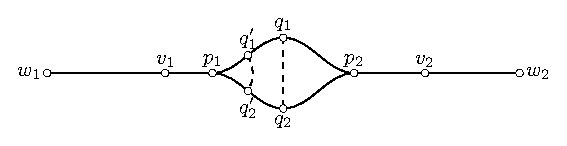
\includegraphics{mppics/pic-30}
\end{figure}

Choose a pair of points $q'_1\in [p_1q_1]$ and $q'_2\in [p_1q_2]$ such that $|p_1-q'_1|\z=|p_1-q'_2|=r'\le r$.
By \ref{cor:splitting-function}, $|q'_1-q'_2|=s(r')$.
Repeating the construction above, we get an $r'$-rhombus for any $r'\in(0,r]$.
\qeds

\subsection*{Self-improvement}

\begin{thm}{Lemma}
Let $M$ be an all-set-homogeneous geodesic space that is not locally uniquely geodesic.
Suppose $r>0$ is sufficiently small.
Then there are $p,q\in M$ and an infinite sequence
$x_1,x_2,\ldots\in M$ such that
\[|p-q|=2\cdot r,
\quad
|p-x_i|=|q-x_i|= r,
\quad\text{and}\quad
|x_i-x_j|=s(r)\] for $ i\ne j$.
\end{thm}

\begin{figure}[b!]
\centering\vskip-0mm

\includegraphics{mppics/pic-40}
\vskip-0mm
\end{figure}

\parit{Proof.}
In the proof we construct and use the configuration of points as in the picture.
Each marked segment has length $r$ times its Roman numeral, and the black points are pairwise at distance $s(r)$.


Choose two points $p$ and $q$ such that $|p-q|=2\cdot r$.
Since $r$ is small, we can extend this pair to a $2\cdot r$-rhombus $p,p',q,q'\in M$;
that is, $|p-p'|=4\cdot r$, $|q-q'|=s(2\cdot r)$, and $|p-q|=|p'-q|=|p-q'|=|p'-q'|=2\cdot r$.
Furthermore, there is a point $z$ such that $p\in \vv zp'\ww$ and $|z-p|=2\cdot r$.

Suppose we have a finite sequence $x_1,\ldots,x_n$ that meets the conditions.
We construct one more point $x_{n+1}$, and induction finishes the proof.

Let $y$ be the midpoint of $[pq']$.
By Corollary~\ref{cor:splitting-function}, $|y-x_i|=s(r)$ for any~$i$.
By the triangle inequality, $|p'-y|=|z-y|=|p'-x_i|=|z-x_i|=3\cdot r$.
Thus an isometry $\iota$ of $M$ maps $z$ to $p'$ and fixes $y,x_1,\ldots,x_n$.
Set $w=\iota(p)$;
the triangle inequality gives
\[|p-w|=2\cdot r
\quad\text{and}\quad
|p-y|=|w-y|=|p-x_i|=|w-x_i|= r\]
for any $i$.
Therefore, there is an isometry $\iota'$ that fixes $p,x_1,\ldots,x_n$ and moves $w$ to $q$.
Note that the point $x_{n+1}=\iota'(y)$ meets all the requirements.
\qeds


\parit{Proof of \ref{prop:unique-geod}.}
Assume, to the contrary, that $M$ is an all-set-homogeneous geodesic space that is not locally uniquely geodesic.
Choose two sufficiently close points $p,q\in M$;
let $r=\tfrac12\cdot|p-q|$.
By the self-improving lemma, the set of midpoints of $p$ and $q$ contains an infinite $s(r)$-equilateral set,
which contradicts \ref{obs:spheres} and~\ref{obs:equilateral}.
\qeds

\section{Spaces with locally unique geodesics}\label{sec:locally unique geodesics}

\subsection*{Local tree}

\begin{thm}{Proposition}\label{prop:loc-tree}
Let $M$ be an all-set-homogeneous geodesic space with locally unique geodesics.
If it has bifurcating geodesics, then $M$ is locally a metric tree;
that is, any point of $M$ has a neighborhood isometric to a metric tree.
\end{thm}

The same proof works for $3$-point-homogeneous spaces.

\parit{Proof.}
Homogeneity and local uniqueness of geodesics imply that there is $R>0$ such that if $|x-y|<R$, then $[xy]$ is uniquely defined.

Let $s$ be the splitting function of $M$; it is defined since $M$ has bifurcating geodesics.%
\footnote{For metric trees we must have $s(t)\equiv2\cdot t$.}

Fix a point $p\in M$ and $r>0$.
Given a point $x$, denote by $x_r$ the point on $[px]$ such that $|p-x_r|=r$;
it is uniquely defined if $r\le |p-x|<R$.
Observe that for any small $\eps>0$ there is $\delta>0$ such that
\[|p-x|,|p-y|\in (r+\eps,R)\  \text{and}\ |x-y|<\delta\ \Rightarrow\  x_r=y_r.\]

\begin{wrapfigure}{o}{40mm}
\centering
\vskip-0mm

\includegraphics{mppics/pic-60}
\vskip-0mm
\end{wrapfigure}

Indeed, let $a=|p-x|$;
we can assume that $a\le |p-y|$.
By \ref{lem:splitting-function}, we can choose $\delta>0$ such that $s(\eps)>2\cdot \delta$.
By the triangle inequality,
\[|x-y|<\delta\quad\Rightarrow\quad|x-y_a|<2\cdot\delta.\]
Suppose $w$ is the splitting point of $[px]$ and $[py]$, and let $b=|w-x|=|w-y_a|$.
Then, by 3-point-homogeneity, $s(b)\le|x-y_a|$,
and hence $b<\eps$ and $x_r=y_r$;
here we assume that $s$ is defined on $[0,R]$.

Choose a geodesic triangle $[pxy]$ in $M$ such that $|p-x|<\tfrac R2$, $|p-y|<\tfrac R2$;
let $r=\tfrac12\cdot(|p-x|+|p-y|-|x-y|)$.
Let us show that $[pxy]$ is a tripod;
once this is done, the statement follows.

If not, then $|p-z|>r$ for any $z\in [xy]$;
note also that $|p-z|<R$.
From above, $z\mapsto z_r$ is locally constant and therefore constant on~$[xy]$.
It follows that $x_r=y_r\in [px]\cap[py]$.
Since $|x-x_r|+|y-y_r|=|x-y|$, we have $[xy]\subset [px]\cup[py]$ --- a contradiction.
\qeds

\subsection*{Global tree}

\begin{thm}{Claim}\label{clm:complete}
Any geodesically complete metric tree $T$ is complete.
\end{thm}

\parit{Proof.}
Assume there is a nonconvergent Cauchy sequence $x_0,x_1,\ldots$ in~$T$.
Let $\ell=\lim |x_0-x_n|$;
note that $\ell>0$.

Denote by $\gamma_n$ the geodesic from $x_0$ to $x_n$ that is parametrized from $x_0$.
If $0\le t<\ell$, then the sequence $\gamma_n(t)$ stabilizes;
that is, $\gamma_i(t)=\gamma_j(t)$ for all sufficiently large $i$ and $j$.
Defining $\gamma_\infty(t)$ as $\gamma_n(t)$ for sufficiently large $n$ produces a geodesic $\gamma_\infty \colon[0,\ell)\to T$.
Since $T$ is geodesically complete, $\gamma_\infty$ extends to $[0,\ell]$, but $x_0,x_1,\ldots$ converge to $\gamma_\infty(\ell)$ --- a contradiction.
\qeds

\parit{Proof of the main statement of \ref{thm:main}.}
Let $M$ be an all-set-homogeneous geodesic space;
by \ref{prop:unique-geod} it has locally unique geodesics.
If geodesics in $M$ do not bifurcate, then, by Birkhoff's theorem, $M$ is classical.
Otherwise, \ref{prop:loc-tree} implies that $M$ is locally a tree.
The existence of a bifurcation implies that the local tree has valence at least $3$ at some (and therefore any) point.

Let us show that $M$ is a metric tree;
in other words, $M$ does not contain an embedded circle \cite[2.2.3]{chiswell}.

Assume the contrary; let $2\cdot R$ be the greatest lower bound of lengths of embedded circles in $M$.
Since $M$ is locally a tree, homogeneity implies that $R>0$.
Absence of embedded circles of length less than $2\cdot R$ implies the following:
\begin{itemize}
\item an $\tfrac R2$-neighborhood of any point in $M$ is a tree with valence at least $3$;
\item if $|x-y|\z<R$, then $[xy]$ is uniquely defined.
\end{itemize}

It follows that any equilateral triangle in $M$ with side $s<R$ is a tripod.
Indeed, choose a point $p$ and three points $x$, $y$, and $z$ in different components of its punctured $\tfrac R2$-neighborhood at distance $\tfrac s2$ from $p$.
Note that $[xyz]$ is a tripod with side~$s$;
by $3$-point-homogeneity the same holds for any triangle with side $s$.

Now choose an embedded circle $\Sigma$ of length slightly above $2\cdot R$.
Choose points $x,y,z$ that divide $\Sigma$ into three equal arcs, say of length $s$;
we can assume  $s<R$.
Note that $|x-y|=s$; otherwise $\Sigma$ together with $[xy]$ would contain an embedded circle of length less than $2\cdot R$,
which is impossible.
It follows that $[xyz]$ is an equilateral triangle of side $s$,
which is not a tripod --- a contradiction.

Thus $M$ is an all-set-homogeneous metric tree;
in particular, it has the same valence at every point.
By \ref{obs:geodesically-complete} and \ref{clm:complete}, $M$ is complete.%
\footnote{Pénélope Azuelos has shown that homogeneity is not sufficient \cite{azuelos2025}:
\emph{there are noncomplete 2-point-homogeneous metric trees  of any valence $n\ge 3$}.}
Thus $M$ is a universal metric tree;
it remains to show that it has finite valence.

Assume the valence is infinite.
Then there is an infinite equilateral set $E\z\subset M$;
indeed, one can take points at a fixed distance in distinct branches of the tree.
This contradicts \ref{obs:equilateral}.
\qeds

\section{Construction of a geodesic}\label{Length-spaces}

The following proposition provides the second statement in \ref{thm:main} modulo the first one.

\begin{thm}{Proposition}\label{prop:ash>geodesic}
A complete all-set-homogeneous length space is geodesic.
\end{thm}

\subsection*{Separated sequence}

Let $M$ be an all-set-homogeneous metric space.
Fix two positive real numbers $a$, $b$ and let $c=a+b$.
Consider the set $\Lambda_{a,c}$ of all $\lambda\ge 0$
such that $a=|u-v|$, $c=|u-w|$, and $b+\lambda=|v-w|$ for some points $u,v,w\in M$;
further assume $\Lambda_{a,c}\ne\varnothing$.

For a pair $s,t\in\Lambda_{a,c}$ we may consider the distance $|s-t|$ induced from $\RR$,
\begin{figure}[ht!]
\centering\vskip-0mm

\includegraphics{mppics/pic-70}
\vskip-0mm
\end{figure}
but there are also two other distances $\theta(s,t)$ and $\Theta(s,t)$ defined as the greatest lower bounds of the values $\ell$ and $L$ for configurations of points shown in the picture.
Formally, we define them as
\begin{align*}
\theta(s,t)
&\df
\inf\set{|v_1-v_2|}{
\substack{
|u-v_i|=a,\ |v_1-w|=b+s,
\\
|u-w|=c,\ |v_2-w|=b+t.
}
},
\\
\Theta(s,t)
&\df
\inf\set{|w_1-w_2|}{
\substack{
|u-v|=a,\ |v-w_1|=b+s,
\\
|u-w_i|=c,\ |v-w_2|=b+t.
}
}.
\end{align*}
The triangle inequalities for $\theta$ and $\Theta$ follow by applying $3$-point-homogeneity
to identify the common triangle in two almost minimizing configurations.

If $M$ is complete, then so are $(\Lambda_{a,c},\theta)$ and $(\Lambda_{a,c},\Theta)$.
Indeed, pass to a subsequence of a Cauchy sequence with summable
successive distances.
By $3$-point-homogeneity, its terms can be represented by points
on a fixed sphere whose successive distances are summable.
Their limit represents the limit in the corresponding metric.

\begin{thm}{Lemma}\label{lem:cauchy-radius}
Let $M$ be a complete all-set-homogeneous length space.
Assume there are no points $u,v,w\in M$ such that
\[
|u-v|=a,\qquad |v-w|=b,\qquad |u-w|=c,
\]
where $a>0$, $b>0$, and $c=a+b<\diam M$.
Then any sequence in $\Lambda_{a,c}$ converging to $0$ contains a subsequence $\lambda_1,\lambda_2,\ldots$
such that
\[\theta(\lambda_i,\lambda_j)>\delta
\quad\text{and}\quad
\Theta(\lambda_i,\lambda_j)>\delta
\]
for some fixed $\delta>0$ and all $i\ne j$.
\end{thm}

\parit{Proof.}
Choose $u,w\in M$ with $|u-w|=c$ and a sequence $v_1,v_2,\ldots$ on the sphere $\S(u,a)$ such that $\lambda_n=|v_n-w|- b$ is the given sequence.

By assumption, $0\notin\Lambda_{a,c}$.
Therefore, the sequence $\lambda_1,\lambda_2,\ldots$ has no $\theta$-Cauchy subsequence.
Consequently, $\lambda_1,\lambda_2,\ldots$ has an infinite $\delta$-separated
subsequence for some $\delta>0$, and the same argument applies to $\Theta$.
\qeds



\subsection*{Descent}

\begin{thm}{Lemma}\label{lem:plus-eps}
Let $M$ be an all-set-homogeneous complete length space.
Suppose $|u-v|<\diam M$.
Then there is a point $w$ such that
$|u-v|+|v-w|=|u-w|$ and $|v-w|>0$ is arbitrarily small.
\end{thm}

\parit{Proof.}
Let $a=|u-v|$; choose $r>0$ so that $a+r<\diam M$.
We can assume $a>0$; the case $a=0$ is immediate.
Suppose $b\in(0,r]$, and $c=a+b$.

Choose $w\in M$ such that $|u-w|=c$.
Let
\[\sigma(b)=\lim_{\lambda\to 0+}\diam(\S(u,a)\cap \B(w,b+\lambda)).\]
By 2-point-homogeneity, $\sigma(b)$ does not depend on the choice of $u$ and $w$.
Note that $\sigma$ is nondecreasing and upper semicontinuous on $(0,r]$; furthermore,
\[
\sigma(b)\le2\cdot b.
\eqlbl{eq:sigma<2b}
\]

Suppose there is no point $w$ with $0<|v-w|\le r$
that meets the requirements;
in other words, $M$ has no triangle with side lengths
$a$, $b$, and $c=a+b$  for $b\in(0,r]$.
By \ref{lem:cauchy-radius}, $\sigma(b)>0$ for any $b\in(0,r]$.

We will show that \emph{$\sigma$ is constant on $(0,r]$} and arrive at a contradiction with~\ref{eq:sigma<2b}.
Note that it is sufficient to show that for each $b\in(0,r]$
there is $b'\in(0,b)$ such that
\[
\sigma(b')\ge\sigma(b).
\eqlbl{sigma=const}
\]

Given $b\in(0,r]$ there is $\delta>0$ such that for any $\eps>0$ there are points $x,y,z\in \S(u,a)$ such that
\begin{align*}
\eps&> \sigma(b)-|y-z|,
&
\lambda(x)&>\lambda(y),
&
\Theta(\lambda(x),\lambda(y))&>\tfrac\delta2,
\\
\eps&>\lambda(x),
&
\lambda(x)&>\lambda(z),
&
\Theta(\lambda(x),\lambda(z))&>\tfrac\delta2,
\end{align*}
where $\lambda(x)\df|w-x|-b$.

Indeed, by \ref{lem:cauchy-radius} we can choose three points $x_1, x_2, x_3\in \S(u,a)$ with $\lambda(x_i)$ from one $\Theta$-separated sequence
such that each distance $|w-x_i|$ is very close to $b$.
Then choose $y,z\in \S(u,a)$ such that
\begin{align*}
|w-y|&<|w-x_i|,
&
|w-z|&<|w-x_i|
\end{align*}
for each $i$, and $|y-z|$ is almost $\sigma(b)$.
Since $\Theta$ is a metric, we may choose $x=x_i$ that meets the conditions.

\begin{wrapfigure}{o}{40mm}
\centering
\vskip-0mm
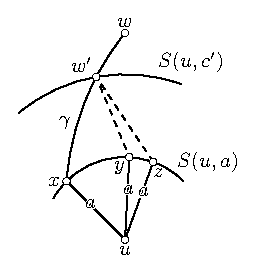
\includegraphics{mppics/pic-80}
\vskip-0mm
\end{wrapfigure}

Choose a curve $\gamma$ from $w$ to $x$ of length sufficiently close to
$|w-x|=b+\lambda(x)$.
Choose $b'>0$ such that $0<b-b'< \tfrac\delta{100}$; let $c'=a+b'$ and $w'\in\gamma\cap \S(u,c')$.
In particular, we have
\[
|w'-w|<\tfrac\delta{10}
\quad\text{and}\quad
|x-w'|<b'+2\cdot\lambda(x).
\]

Let $\rho$ be a reflection interchanging $x$ with $y$;
note that $\rho(u)=u$.
Since
\begin{align*}
\tfrac\delta2&<\Theta(\lambda(x),\lambda(y))
\le
\\
&\le
|w-\rho(w)|=
\\
&=
2\cdot\inf\set{|w-h|}{h\in \Bis(x,y)},
\end{align*}
the point $w$ lies at distance at least $\tfrac\delta{10}$ from $\Bis(x,y)$.
Since $|w'-w|<\tfrac\delta{10}$, both points $w$ and $w'$ lie on the same side of $\Bis(x,y)$, and
\[|w-x|>|w-y|
\quad\Rightarrow\quad
|w'-x|>|w'-y|.\]
Therefore,
\[y\in \S(u,a)\cap \B(w',b'+2\cdot\lambda(x)),\]
and similarly,
\[z\in \S(u,a)\cap \B(w',b'+2\cdot\lambda(x)).\]
Thus \ref{sigma=const} follows.
\qeds

\subsection*{Expanding collinear sets}

\begin{thm}{Lemma}\label{cor:plus-one}
Let $f$ be a distance-preserving map from a finite set of real numbers $X$ into an all-set-homogeneous length space $M$.
Given three consecutive numbers $t_{i-1},t_i,t_{i+1}\in X$, set $t_i'=t_{i-1}-t_i +t_{i+1}$.
Then the map $f$ can be extended to a distance-preserving map on $X\cup\{t_i'\}$.
\end{thm}

\parit{Proof.}
Set $x_i=f(t_i)$ and let $f(t_i')\df x_i'\df\rho(x_i)$, where $\rho$ is the reflection that swaps $x_{i-1}$ and $x_{i+1}$.
We can assume $|x_{i-1}-x_i|\ge |x_i-x_{i+1}|$.
Then
\[|x_{i-1}-x'_i|+|x'_i-x_i|+|x_i-x_{i+1}|=|x_{i-1}-x_{i+1}|;\]
the triangle inequality gives the lower bound, and an almost shortest path from
$x_{i-1}$ to $x_i$ gives the upper bound.
Hence the statement follows.
\qeds

\parit{Proof of \ref{prop:ash>geodesic}.}
Let $M$ be a complete all-set-homogeneous length space.
Choose two points $u,v\in M$ and let $a=|u-v|$.
Assume $a<\diam M$.

Let $X$ be a finite set of real numbers $0=t_1<\ldots<t_n=a$,
and let $f\:X\to M$ be a distance-preserving map such that $u=f(0)$ and $v=f(a)$.

By \ref{lem:plus-eps}, we can choose a point $w\in M$ such that $|u-v|+|v-w|=|u-w|$
and $b=|v-w|>0$ is arbitrarily small.
Let $c=a+b=|u-w|$ and let $f(c)=w$;
note that $f$ is still distance-preserving.

Applying \ref{cor:plus-one}, we can propagate a short gap from right to left,
extending $f$ to a larger subset of $[0,c]$ such that consecutive points are at distance at most~$b$.
Then we can pass to the intersection of the enlarged domain with $[0,a]$ and repeat the procedure for a smaller $b>0$.

Repeating this procedure, we extend $f$ to a distance-preserving map on a dense set of $[0,a]$.
By completeness of $M$, the map $f$ extends to a geodesic from $u$ to $v$.
Thus a geodesic $[uv]$ exists if $|u-v|<\diam M$.

If $a=\diam M$, we can choose a sequence of geodesics $[uv_1],[uv_2],\ldots$ such that
$|u-v_n|\to a$ as $n\to\infty$.
By 2-point-homogeneity, we can assume that they are nested: $[uv_1]\subset[uv_2]\subset\ldots$
Taking their union and passing to its closure gives a geodesic of length $a$.
Now, by 2-point-homogeneity, $M$ is geodesic.
\qeds


\parbf{Acknowledgements.}
We thank Alexander Lytchak for his help.
The proof was developed in collaboration with AI (GPT-6 Astra).

{\sloppy
\printbibliography[heading=bibintoc]
\fussy
}

\end{document}

